\section{Auswertung}
\label{sec:Auswertung}
{\footnotesize \textit{Jonat$\hbar$an Kriewald}}

\subsection{Das Magnetfeld}
Um die magentische Feldstärke bei der Probe zu ermitteln, wurde die gemessene Feldstärke gegen den Abstand zur Probe in beide Richtungen geplottet.
Diese sind in Abbildung \ref{fig:plot} zu sehen.
\begin{figure}
  \centering
  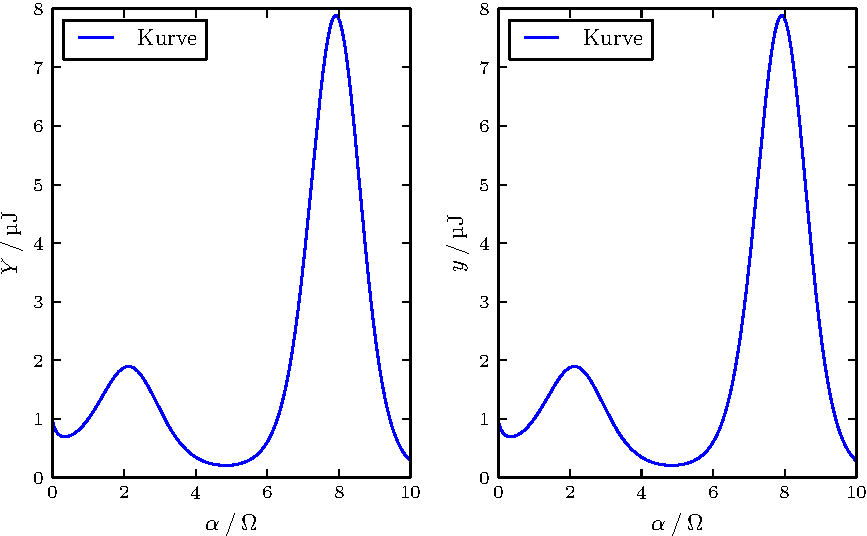
\includegraphics{pc/plot.pdf}
  \caption{Das Magnetfeld.}
  \label{fig:plot}
\end{figure}
Die Messwerte sind in Tabelle \ref{tab:B} eingetragen.
Als Feldstärke an der Probe wird der Mittelwert von $B = \SI{447.5}{\milli\tesla}$ angenommen.
\begin{table}[h]
\centering
\caption{Das Magnetfeld.}
\sisetup{%uncertainty-seperator = {\,},
table-number-alignment = center,
table-unit-alignment = center,
%table-figures-integer = 1,
%table-figures-decimal = 1,
table-auto-round = true
}
\begin{tabular}{  S[table-format= 1.0] 
 S[table-format= 3.0] 
 S[table-format= 3.0] 
}
\toprule
{$\text{Abstand zu Probe}\:/\:\si{\milli\meter}$}
&{$\text{Feldstärke positiver Polung}\:/\:\si{\milli\tesla}$}
&{$\text{Feldstärke negativer Polung}\:/\:\si{\milli\tesla}$} \\
 \midrule
-9.0&336.0&341.0\\
-8.0&336.0&391.0\\
-7.0&358.0&414.0\\
-6.0&393.0&428.0\\
-5.0&412.0&436.0\\
-4.0&425.0&443.0\\
-3.0&433.0&447.0\\
-2.0&438.0&450.0\\
-1.0&442.0&450.0\\
0.0&444.0&451.0\\
1.0&445.0&451.0\\
2.0&443.0&448.0\\
3.0&439.0&444.0\\
4.0&434.0&438.0\\
5.0&426.0&430.0\\
6.0&414.0&417.0\\
7.0&400.0&403.0\\
8.0&377.0&380.0\\
9.0&342.0&347.0\\
10.0&298.0&298.0\\
11.0&243.0&243.0\\
12.0&195.0&179.0\\
\bottomrule
\end{tabular}
\label{tab:B}
\end{table}

\subsection{Messung der Faraday-Rotation}
Die Proben an denen die Faraday-Rotation gemessen wurde, sind 2 dotierte und ein hochreiner GaAs Halbleiter.
Die dotierten Proben haben eine Ladungsträgerdichte von $N_1 =  1{,}2 \cdot 10^{18} \si{\per\cubic\centi\meter}$ respektive $N_2 = 2{,}8 \cdot 10^{18} \si{\per\cubic\centi\meter}$.
Die Proben haben Dicken von $d_1 = \SI{1.36}{\milli\meter}$, $d_2 = \SI{1.296}{\milli\meter}$ und $d_\text{rein} = \SI{5.11}{\milli\meter}$.
Die bei den unterschiedlich ausgerichteten Magnetfelder gemessenen Rotationswinkel sind in den Tabellen \ref{tab:th1} - \ref{tab:th3} zu sehen.
Der Differenzwinkel wurde dabei mit der Probendicke normiert.
Dieser wird nach 
\begin{equation}
	\theta_\text{f} = \frac{1}{2}(\theta_- -\theta_+)
\end{equation}
gebildet und benötigt, da durch die Umpolung des Magnetfeldes der doppelte Winkel gemessen wurde.
\begin{table}[h]
\centering
\caption{Werte Probe 1}
\sisetup{%uncertainty-seperator = {\,},
table-number-alignment = center,
table-unit-alignment = center,
%table-figures-integer = 1,
table-figures-decimal = 5,
table-auto-round = true
}
\begin{tabular}{  S[table-format= 3.2] 
 S[table-format= 3.2] 
 S[table-format= 3.2] 
 S[table-format= 3.4] 
}
\toprule
{$\lambda \:/\: \si{\micro\meter}$}
&{$\theta_{+}\:/\: °$}
&{$\theta_{-}\:/\: °$}
&{$\frac{\theta_{\text{f}}}{d}\:/\: \si{\radian\per\milli\meter}$} \\
 \midrule
1.06&127.83&140.16&0.0532276951652\\
1.29&131.92&138.92&0.0188732435374\\
1.45&131.58&135.67&0.003189364688\\
1.96&269.0&277.92&0.0445820418665\\
2.16&138.16&145.16&0.0386490877038\\
2.34&173.58&181.0&0.039926641794\\
2.51&209.33&201.08&0.0479507212037\\
2.65&145.25&152.2&0.0303701002144\\
\bottomrule
\end{tabular}
\label{tab:th1}
\end{table}

\begin{table}[h]
\centering
\caption{Werte Probe 2}
\sisetup{%uncertainty-seperator = {\,},
table-number-alignment = center,
table-unit-alignment = center,
%table-figures-integer = 1,
table-figures-decimal = 5,
table-auto-round = true
}
\begin{tabular}{  S[table-format= 3.2] 
 S[table-format= 3.2] 
 S[table-format= 3.2] 
 S[table-format= 3.4] 
}
\toprule
{$\lambda \:/\: \si{\micro\meter}$}
&{$\theta_{+}\:/\: °$}
&{$\theta_{-}\:/\: °$}
&{$\frac{\theta_{\text{f}}}{d}\:/\: °\si{\radian\per\milli\meter}$} \\
 \midrule
1.06&128.0&141.16&0.0627235474454\\
1.29&131.33&140.5&0.0357030910132\\
1.45&132.33&138.67&0.0196357974225\\
1.96&268.0&276.5&0.0445804575081\\
2.16&135.5&150.16&0.0924459783642\\
2.34&172.58&183.5&0.0658451614321\\
2.51&197.33&208.75&0.071910181637\\
2.65&142.5&154.42&0.0660379694823\\
\bottomrule
\end{tabular}
\label{tab:th2}
\end{table}

\begin{table}[h]
\centering
\caption{Werte Probe 3}
\sisetup{%uncertainty-seperator = {\,},
table-number-alignment = center,
table-unit-alignment = center,
%table-figures-integer = 1,
table-figures-decimal = 5,
table-auto-round = true
}
\begin{tabular}{  S[table-format= 3.2] 
 S[table-format= 3.2] 
 S[table-format= 3.2] 
 S[table-format= 3.4] 
}
\toprule
{$\lambda \:/\: \si{\micro\meter}$}
&{$\theta_{+}\:/\: °$}
&{$\theta_{-}\:/\: °$}
&{$\frac{\theta_{\text{f}}}{d}\:/\: \si{\radian\per\milli\meter}$} \\
 \midrule
1.06&129.0&144.16&0.0258896198241\\
1.29&125.67&140.92&0.0260433180948\\
1.45&126.92&140.42&0.0230547406085\\
1.96&268.92&276.33&0.0126544909562\\
2.16&140.0&143.67&0.00626747392839\\
2.34&173.5&178.0&0.00768491353618\\
2.51&210.0&212.92&0.0049866550057\\
2.65&147.67&156.0&0.0142256288347\\
\bottomrule
\end{tabular}
\label{tab:th3}
\end{table}

Die Messerergebnisse werden gegen die Wellenlänge $\lambda$ in Abbildung \ref{fig:rot} aufgetragen.
\begin{figure}
	\centering
	\includegraphics{pc/rot.pdf}
	\caption{Gemessene Rotationswinkel.}
	\label{fig:rot}
\end{figure}
Um die effektive Masse der Elektronen zu ermitteln, muss die Differenz der Rotationswinkel der dotierten Proben mit dem der reinen Probe berechnet werden. Die so resultierenden Rotationswinkel sind in Tabelle \ref{tab:thr} eingetragen.
Diese werden in Abb. \ref{fig:p} gegen $\lambda²$ aufgetragen und mit einer Ursprungsgerade nach Gleichung \eqref{eqn:formel} gefittet.
\begin{figure}
	\centering
	\includegraphics{pc/p.pdf}
	\caption{Messwerte und fit.}
	\label{fig:p}
\end{figure}
Mit dem Fitparameter $a_1 = \SI{0.007\pm0.002}{\per\cubic\micro\meter}\cdot 10^{-3}$ und $a_2 = \SI{0.013\pm0.002}{\per\cubic\micro\meter}\cdot10^{-3}$ als Geradensteigung ergeben sich mit
\begin{equation}
	m_{*i} = \sqrt{\frac{e³N_i B}{8\pi² n \epsilon_0 c³ a_i}}
\end{equation}
die effektiven Massen
\begin{align}
	m_{*1} &= \SI{6.9\pm0.8}{\kilo\gram}\cdot10^{-32} &= \SI{0.076\pm0.008}{m_e}\\
	m_{*2} &= \SI{8.0\pm0.6}{\kilo\gram}\cdot10^{-32} &= \SI{0.088\pm0.007}{m_e}\text.
\end{align}
Hierbei wird ein Brechungsindex von $n=\SI{3.4}{}$ angenommen.
\begin{table}[h]
\centering
\caption{Resultierender Winkel Probe 1 und 2}
\sisetup{%uncertainty-seperator = {\,},
table-number-alignment = center,
table-unit-alignment = center,
%table-figures-integer = 1,
table-figures-decimal = 5,
table-auto-round = true
}
\begin{tabular}{  S[table-format= 3.2] 
 S[table-format= 3.4] 
 S[table-format= 3.4] 
}
\toprule
{$\lambda \:/\: \si{\micro\meter}$}
&{$\theta_1 \:/\: \si{\radian\per\milli\metre}$}
&{$\theta_2 \:/\: \si{\radian\per\milli\metre}$} \\
 \midrule
1.06&0.0532276951652&0.0627235474454\\
1.29&0.0188732435374&0.0357030910132\\
1.45&0.003189364688&0.0196357974225\\
1.96&0.0445820418665&0.0445804575081\\
2.16&0.0386490877038&0.0924459783642\\
2.34&0.039926641794&0.0658451614321\\
2.51&0.0479507212037&0.071910181637\\
2.65&0.0303701002144&0.0660379694823\\
\bottomrule
\end{tabular}
\label{tab:thr}
\end{table}


